\section{The Sprout Algorithm}
\label{s:sprout}

Motivated by the varying capacity of cellular networks (as captured in
Figure~\ref{fig:skypevssprout}), we designed Sprout to compromise
between two desires: achieving the highest possible throughput, while
preventing packets from waiting too long in a network queue.

From the transport layer's perspective, a cellular network behaves
differently from the Internet's traditional infrastructure in several
ways. One is that endpoints can no longer rely on packet drops to
learn of unacceptable congestion along a network path
(\cite{bufferbloat}), even after delays reach ten seconds or more. We
designed Sprout not to depend on packet drops for information about
the available throughput and the fullness of in-network queues.

Another distinguishing feature of cellular links is that users are
rarely subject to standing queues accumulated by other users, because
a cellular carrier generally provisions a separate uplink and downlink
queue for each device in a cell. In a network where two independent
users share access to a queue feeding into a bottleneck link, one user
can inflict delays on another. No end-to-end protocol can provide
low-delay service when a network queue is already full of somebody
else's packets. But when queueing delays are largely self-inflicted,
an end-to-end approach may be possible.\footnote{An end-to-end
  approach may also be feasible if all sources run the same protocol,
  but we do not investigate that hypothesis here.}

In our measurements, we found that estimating the capacity (by which
we mean the maximum possible bit rate or throughput) of cellular links
is challenging, because they do not have a directly observable rate
{\em per se}. Even in the middle of the night, when average throughput
is high and an LTE device may be completely alone in its cell, packet
arrivals on a saturated link do not follow an observable
isochronicity. This is a roadblock for packet-pair techniques
(\cite{packetpair}) and other schemes to measure the available
throughput.

Figure~\ref{f:vzinter} illustrates the {\em interarrival} distribution
of 1.2 million MTU-sized packets received at a stationary cell phone
whose downlink was saturated with these packets. For the vast majority
of packet arrivals (the 99.99\% that come within 20~ms of the previous
packet), the distribution fits closely to a memoryless point process,
or Poisson process, but with fat tails suggesting the impact of
channel quality-dependent scheduling, the effect of other users, and
channel outages, that yield interarrival times between 20 ms and as
long as four seconds.  Such a ``switched'' Poisson process produces a
$1/f$ distribution, or {\em flicker noise}. The best fit is shown in
the plot.\footnote{We can't say exactly why the distribution should
  have this shape, but physical processes could produce such a
  distribution. Cell phones experience fading, or random variation of
  their channel quality with time, and cell towers attempt to send
  packets when a phone is at the apex of its channel quality compared
  with a longer-term average. }
%\anirudh{TWhat is the -3.27 in the exponent of t ? Maybe a desc of flicker noise would help ?}


\begin{figure}
\caption{Interarrival times on a Verizon LTE downlink, with receiver
  stationary, fit to a $1/f$ noise distribution.}

\hspace{\baselineskip}

\def\svgwidth{\columnwidth}\input{vz-inter.pdf_tex}

\label{f:vzinter}

\end{figure}

A Poisson process has an underlying rate $\lambda$, which may be
estimated by counting the number of bits that arrive in a long
interval and dividing by the duration of the interval. In practice,
however, the rate of these cellular links varies more rapidly than the
averaging interval necessary to achieve an acceptable estimate.

Sprout needs to be able to estimate the link speed, both now and in
the future, in order to predict how many packets it is safe to send
without risking their waiting in a network queue for too long. An
uncertain estimate of future link speed is worth more caution than a
certain estimate, so we need to quantify our uncertainty as well as
our best guess.

We therefore treat the problem in two parts. We model the link and
estimate its behavior at any given time, preserving our full
uncertainty. We then use the model to make forecasts about how many
bytes the link will be willing to transmit from its queue in the near
future. Most steps in this process can be precalculated at program
startup, meaning that CPU usage (even at high throughputs) is less
than 5\% of a current Intel or AMD PC microprocessor. We have not
tested Sprout on a CPU-constrained device or tried to optimize it
fully.

\subsection{Inferring the rate of a varying Poisson process}

We model the link as a doubly-stochastic process, in which the
underlying $\lambda$ of the Poisson process itself varies in Brownian
motion\footnote{This is a Cox model of packet
  arrivals~\cite{Cox84,Paxson95}.} with a noise power of $\sigma$
(measured in units of packets per second per
$\sqrt{\mbox{second}}$). In other words, if at time $t = 0$ the value
of $\lambda$ was known to be 137, then when $t = 1$ the probability
distribution on $\lambda$ is a normal distribution with mean 137 and
standard deviation $\sigma$.  The larger the value of $\sigma$, the
more quickly our knowledge about $\lambda$ becomes useless and the
more cautious we have to be about inferring the link rate based on
recent history.

Figure \ref{f:sprout-model} illustrates this model. We refer to the
Poisson process that dequeues and delivers packets as the service
process, or packet-delivery process.

The model has one more behavior: if $\lambda = 0$ (an outage), it
tends to stay in an outage. We expect the outage's duration to follow
an exponential distribution $\exp\left[-\lambda_z\right]$. We call
$\lambda_z$ the outage escape rate. This serves to match the behavior
of real links, which do have ``sticky'' outages in our experience.

In our implementation of Sprout, $\sigma$ and $\lambda_z$ have fixed
values that are the same for all runs and all networks. ($\sigma$ =
200 MTU-sized packets per second per~$\sqrt{\mbox{second}}$, and $\lambda_z =
1$.) These values were chosen based on preliminary empirical
measurements, but the entire Sprout implementation including this
model was frozen before we collected our measurement 3G and LTE traces
and has not been tweaked to match them.

A more sophisticated system would allow $\sigma$ and $\lambda_z$ to
vary slowly with time to better match more- or less-variable networks,
Currently, the only parameter allowed to change with time, and the
only one we need to infer in real time, is $\lambda$---the underlying,
variable link rate.

\begin{figure}
  \caption{Sprout's model of the network path. A Sprout session
    maintains this model separately in each direction.}

\hspace{\baselineskip}

\noindent \def\svgwidth{\columnwidth}\large\input{sprout-model.pdf_tex}

\label{f:sprout-model}

\end{figure}


To solve this inference problem tractably, Sprout discretizes the
space of possible rates, $\lambda$, and assumes that:

\begin{itemize}

\item $\lambda$ is one of 256 discrete values sampled uniformly from 0
  to 1000 MTU-sized packets per second (11 Mbps; larger than
  the maximum rate we observed).
%  \anirudh{We could add a footnote saying why we picked 11Mbps as the max }

\item At program startup, all values of $\lambda$ are equally
  probable.

\item An inference update procedure will run every 20~ms, known as a
  ``tick''. (We pick 20 ms for computational efficiency.)

%  \anirudh{We run it every 20ms, only for computational
%    efficiency right ? I think we should mention that so that people
%    don't ask if we have tried other tick intervals .}

\end{itemize}

By assuming an equal time between updates to the probability
distribution, Sprout can precompute the normal distribution with
standard deviation to match the Brownian motion per tick.

\subsection{Evolution of the probability distribution on $\lambda$}

Sprout maintains the probability distribution on $\lambda$ in 256
floating-point values summing to unity. At every tick, Sprout does
three things:

\begin{enumerate}

\item It \emph{evolves} the probability distribution to the current
  time, by applying Brownian motion to each of the 255 values $\lambda
  \not = 0$. For $\lambda = 0$, we apply Brownian motion, but also use
  the outage escape rate to bias the evolution towards remaining at
  $\lambda = 0$.
  
\item It \emph{observes} the number of bytes that actually came in
  during the most recent tick. This step multiplies each probability
  by the likelihood that a Poisson distribution with the corresponding
  rate would have produced the observed count during a tick. Suppose
  the duration of a tick is $\tau$ seconds (e.g., $\tau = 0.02$) and
  $k$ bytes were observed during the tick. Then, Sprout updates the
  (non-normalized) estimate of the probabilities $F$:
 $$
 F(x) \leftarrow
 \Pr_{\textrm{old}}(\lambda = x) \frac{(x \cdot \tau)^k}{k!}  \exp[-x \cdot \tau].
 $$

\item It \emph{normalizes} the 256 probabilities so that they sum to unity:
$$
\Pr_{\textrm{new}}(\lambda = x) \leftarrow \frac{F(x)}{\sum_i F(i)} .
$$
\end{enumerate}

These steps constitute Bayesian updating of the probability
distribution on the current value of $\lambda$.

One important practical difficulty concerns how to deal with the
situation where the queue is underflowing because the sender has not
sent enough. To the receiver, this case is indistinguishable from an
outage of the service process, because in either case the receiver
doesn't get any packets.

We use two techniques to solve this problem. First, in each outgoing
packet, the sender marks its expected ``time-to-next'' outgoing
packet.  For a flight of several packets,
the time-to-next will be zero for all but the last packet. When the
receiver's most recently-received packet has a nonzero time-to-next,
it skips the ``observation'' process described above until this timer
expires. Thus, this ``time-to-next'' marking allows the receiver to
avoid mistakenly observing that zero packets were deliverable during
the most recent tick, when in truth the queue is simply empty.

Second, the sender sends regular heartbeat packets when idle to help
the receiver learn that it is not in an outage. Even one tiny packet
does much to dispel this ambiguity.

\subsection{Making the packet delivery forecast}

Given a probability distribution on $\lambda$, Sprout's receiver would
like to predict how much data it will be safe for the sender to send
without risking that packets will be stuck in the queue for too
long. No forecast can be absolutely safe, but for typical interactive
applications we would like to bound the risk of a packet's getting
queued for longer than the sender's tolerance to be less than 5\%.

To do this, Sprout calculates a \emph{packet delivery forecast}: a
cautious estimate, at the 5th percentile, of how many bytes will
arrive at its receiver during the next eight ticks, or 160~ms.

It does this by \emph{evolving} the probability distribution forward
(without observation) to each of the eight ticks in the forecast.  At
each tick, Sprout sums over each $\lambda$ to find the probability
distribution of the cumulative number of packets that will have been
drained by that point in time. We take the 5th percentile of this
distribution as the cautious forecast for each tick. Most
of these steps can also be precalculated, so the only work at
runtime is to take a weighted sum over each $\lambda$.

\subsection{The control protocol}

The Sprout receiver sends a new forecast to the sender by piggybacking
it onto its own outgoing packets.

In addition to the predicted packet deliveries, the forecast also
contains a count of the total number of bytes the receiver has
received so far in the connection or has written off as lost. This
total helps the sender estimate how many bytes are in the queue (by
subtracting it from its own count of bytes that have been sent).

In order to help the receiver calculate this number and detect losses
quickly, the sender includes two fields in every outgoing packet: a
sequence number that counts the number of bytes sent so far, and a
``throwaway number'' that specifies the sequence number offset of the
\emph{most recent} sent packet that was sent more than 10~ms prior.

The assumption underlying this method is that while the network may
reorder packets, it will not reorder two packets that were sent more
than 10~ms apart. Thus, once the receiver actually gets a packet from
the sender, it can mark all bytes (up to the sequence number of the
first packet sent within 10~ms) as received or lost, and only keep
track of more recent packets.

\subsection{Using the forecast}

\begin{figure}
\caption{Calculating the window sizes from the forecast. The forecast
  represents the receiver's estimate of a lower bound (with 95\%
  probability) on the cumulative number of packets that will be
  delivered over time.}

\hspace{\baselineskip}

\noindent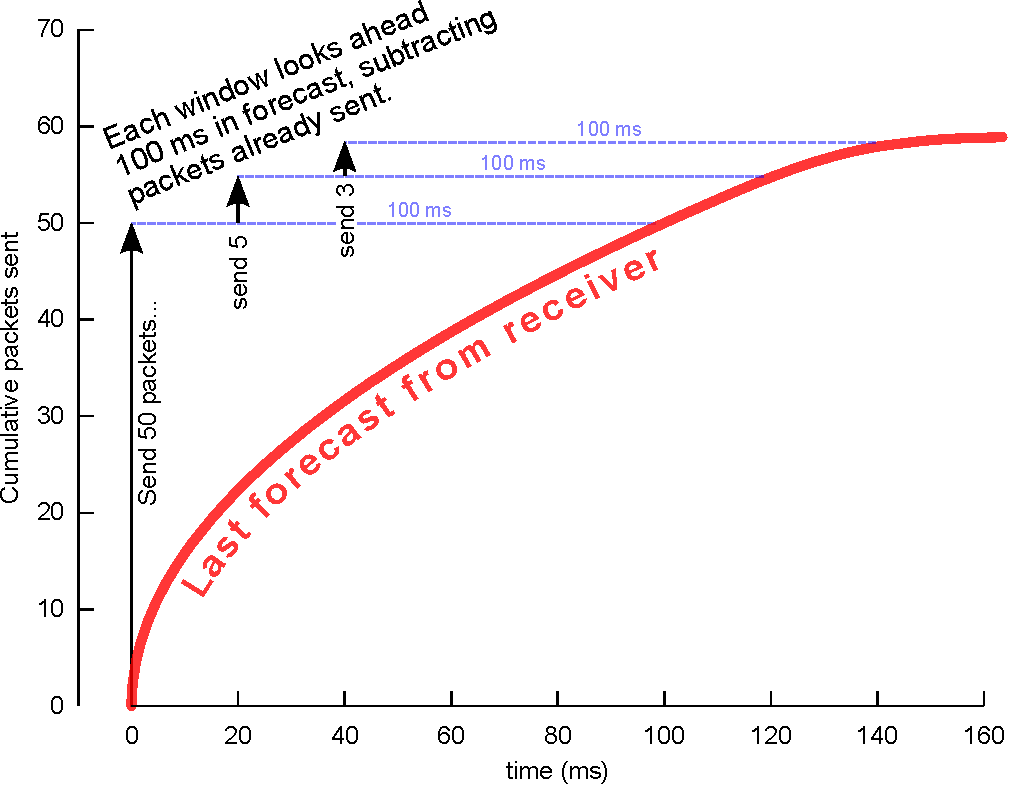
\includegraphics[width=\columnwidth]{forecast.pdf}

\label{f:forecast}

\end{figure}

The Sprout sender uses the most recent forecast it has obtained from the
receiver to calculate a window size---the number of bytes it may
safely transmit, while ensuring that every packet has 95\% probability
of clearing the queue within 100~ms (a conventional standard for
interactivity). Upon receipt of the forecast, the sender timestamps it and
estimates the current queue occupancy, based on the difference between
the number of bytes it has sent so far and the ``received-or-lost''
sequence number in the forecast.

The sender maintains its estimate of queue occupancy going
forward. For every byte it sends, it increments the estimate. Every
time it advances into a new tick of the 8-tick forecast, it decrements
the estimate by the amount of the forecast, bounding the estimate
below at zero packets.

To calculate a window size that is safe for the application to send,
Sprout looks ahead five ticks (100~ms) into the forecast's future, and
counts the number of bytes expected to be drained from the queue over
that time. Then it subtracts the current queue occupancy
estimate. Anything left over is ``safe to send''---bytes that we
expect to be cleared from the queue within 100~ms, even taking into
account the queue's current contents. This evolving window size
governs how much the application may transmit. Figure~\ref{f:forecast}
illustrates this process schematically.

As time passes, the sender may look ahead further and further into the
forecast (until it reaches 160~ms), even without receiving an update
from the receiver. In this manner, Sprout combines elements of pacing
with window-based flow control.
